%!TEX TS-program = XeLaTeX
\documentclass[12pt]{article}
\usepackage[top=1in, bottom=1in, left=1in, right=1in]{geometry}

%%%
%% Needed for fonts in xelatex to work
%%%
% NOTE: I actually use XeLaTeX, which allows me to get the fonts
% exactly the way that I want them. For proposals, this means
% I can use Times New Roman instead of the default Computer
% Modern. I actually like Computer Modern, but since Arial
% is what the solicitation suggests there's no point in throwing off a reviewer
% with an unexpected font, particularly one with such a
% polarizing reaction in readers. Never upset the reviewrers, I
% always say.
%
% What's the point of this bit of rambling? If you do not want to use
% XeLaTeX and would rather stick to good old LaTeX, then you
% need to comment out the next few lines of font packages and
% font commands.
%
% If you want to use XeLaTeX but want different fonts, then you
% just need to change the name in the argument for \setmainfont.
% Make sure that the font you use is loaded on
% your machine and your TeX distribution knows how to find it.
% See Google if you need to learn more about this.
%
\usepackage{fontspec}
\setmainfont{Arial}

%%%
%% Packages that I use on a regular basis.
%%%
% Of course, you are likely to need some math typesetting so these
% three packages have you covered.
\usepackage{amssymb}
\usepackage{amsmath}
\usepackage{latexsym}
% I use color, graphicx, and epstopdf to read in PDFs for my figures.
\usepackage{color}
\usepackage{graphicx}
% \usepackage{epstopdf}
% I don't remember why threeparttable and setspace is here. Inertia.
\usepackage{threeparttable}
\usepackage{setspace}
% \doublespacing
%%%
%% Some packages to handle the figures and captions
%%%
\usepackage[labelfont=bf]{caption}
\usepackage{subcaption}
\usepackage{wrapfig}

%%%
%% Packages and settings for my bibliography.
%%%
% apa_with_doi is a style I created to keep DOI in the bibliography
% but strip out URLs. There are a lot of other styles you can
% find for natbib. Again, Google is your friend.
% Author name and year references, i.e., Author (year):
%\usepackage{natbib}
%\bibliographystyle{apa_with_doi}
% Numbered references:
\usepackage[numbers,super]{natbib}
\bibliographystyle{unsrtnat}


%%%
%% Packages and commands to build my table of contents (TOC).
%%%
%% The trick was getting the References included properly.
%% Also, some of my table of contents entry have no page number
%% because those pages are generated separately by my institute.
%% Nothing to be done about that. You may or may not have the
%% same problem, so you may or may not have to tweak this.
\usepackage[nottoc,numbib]{tocbibind}
\renewcommand{\tocbibname}{References}
\usepackage{tocloft}
\renewcommand{\cftsecleader}{\cftdotfill{\cftdotsep}}

%%%
%% These commands get the spacing around the title and section titles right.
%%%
% I tightened up the spacing. The LaTeX default is just too roomy.
% This spacing is still clean and legible, just not so free with the
% whitespace between sections.
%
% First the title.
\usepackage{titling}
\setlength{\droptitle}{-50pt}
\pretitle{\begin{center}\Large\bfseries\vspace{0ex}}%
\posttitle{\end{center}\Large\vspace{-2ex}}%
\preauthor{\begin{center}\large}%
\postauthor{\end{center}\large\vspace{-3ex}}%
\predate{\begin{center}\large}%q
\postdate{\end{center}\large\vspace{-6ex}}%
% Now the section headings.
\usepackage[noindentafter]{titlesec}
\titleformat{\section}{\large\bfseries}{\thesection}{1em}{}
\titlespacing{\section}{0pt}{18pt plus 2pt minus 2pt}{4pt plus 2pt minus 2pt}[0pt]
\titlespacing{\subsection}{0pt}{16pt plus 2pt minus 2pt}{4pt plus 2pt minus 2pt}[0pt]
\titlespacing{\subsubsection}{0pt}{14pt plus 2pt minus 2pt}{4pt plus 2pt minus 2pt}[0pt]

%%%
%% These commands get the lists to work the way that I want them to.
%%%
% i.e. I want less space wrapping around the list.
\usepackage{enumitem}
\setlist{nolistsep}
\setlist[2]{noitemsep}
\setlist[1]{noitemsep}

%%%
%% Commands for making the tables.
%%%
\usepackage{booktabs}
\usepackage{multirow}
\usepackage{array}


%%%
%%% Formatting urls
%%%
\usepackage{url}
\urlstyle{rm}

%% The lineno packages adds line numbers. Start line numbering with
%% \begin{linenumbers}, end it with \end{linenumbers}. Or switch it on
%% for the whole article with \linenumbers after \end{frontmatter}.
\usepackage{lineno}

%% In order to have a caption to the side of a figure or table, use the
%% 'sidecap' package.
\usepackage[rightcaption]{sidecap}
\sidecaptionvpos{figure}{t}

\usepackage{wrapfig}


%% For more control of the enumeration environment (lists with numbers)
%% use the enumitem package.
%\usepackage{enumitem}

%% Also, to reset the numbering of enumerate, use the following:
%\setenumerate[0]{label=\alph*.}

% To deal with figures all alone on a page.
\renewcommand{\floatpagefraction}{.8}%

% To use symbols for the footnotes:
\renewcommand{\thefootnote}{\fnsymbol{footnote}}

% set up the page numbers as 1-N, 2-N, ...
\numberwithin{page}{section}
\renewcommand{\thepage}{\thesection-\arabic{page}}

% https://tex.stackexchange.com/questions/210871/latex-page-numbering-by-section
%this does not seem to work, just hard code it :(
% not sure if there is something else in this template that is breaking it
% or things have changed in the last 6 years?
%\usepackage{etoolbox}
%\makeatletter
%% Make sure that page starts from 1 with every \section
%\patchcmd{\@sect}% <cmd>
%  {\protected@edef}% <search>
%  {\def\arg{#1}\def\arg@{section}%
%   \ifx\arg\arg@\stepcounter{page}\fi%
%   \protected@edef}% <replace>
%  {}{}% <success><failure>
%\makeatother

%% Finally, we get to the document.
\begin{document}
\title{Improving the Foundations and Maintenance of Matplotlib}
\author{Dr. Thomas A Caswell}
\date{}
\maketitle

% First, let's get that TOC in there. NASA likes it.
\setcounter{tocdepth}{2}
\tableofcontents
\thispagestyle{empty}
% Let's leave this TOC alone on this page and start a new one for
% proposal body.
\newpage

\section{Scientific/Technical/Management (S/T/M)}
% Let's reset the page counter.
\setcounter{page}{1}
% the subsection are a combination of the lines labeled "Content" in
% Table 1 (on ROSES-20 SoS-51) and the text in E.7.3 (on E.7-2 -
% E.7-3) describing what needs to be in the proposal.

% not sure that this order is right, but I think we need to hit all of
% these points.  Maybe want to rename the section headings or merge
% some of them?
\subsection{Description of software and relevance to SMD}

Billions of dollars of SMD funding, across all 4 SMD divisions,
critically relies on the scientific Python ecosystem (SPE) for data
analysis, scientific computation and visualization.  This includes
flagship missions like the Hubble Space Telescope, the James Web Space
Telescope, and the Curiosity rover
Mastcam\cite{https://doi.org/10.1002/2016EA000219}.  The Scientific
Python Ecosystem is a loosely defined community of projects and
programmers with the common goal of advancing science through the use
of the Python programming language.  This development is largely
volunteer work or work that is sponsored implicitly by specific
science projects.  SPE, shown with a rough schematic in Figure
\ref{fig:ecosystem}, has a core of general purpose domain-agnostic
tools, like NumPy\cite{Harris2020} and SciPy\cite{Virtanen2020}. In
the next ring is specialized, but still domain agnostic tools like
Matplotlib\cite{Hunter:2007}, the fundamental data visualization
library for the SPE, and advanced data structures like Pandas and
XArray.  The outer rings are increasingly domain specific tools, like
AstroPy\cite{robitaille2013astropy} and
SunPy\cite{sunpy_community2020}.  This layered approach gives
scientists and engineers convenient and powerful high level tools
while enabling direct access to the underlying libraries when needed.


\begin{wrapfigure}{r}{0.5\textwidth}
  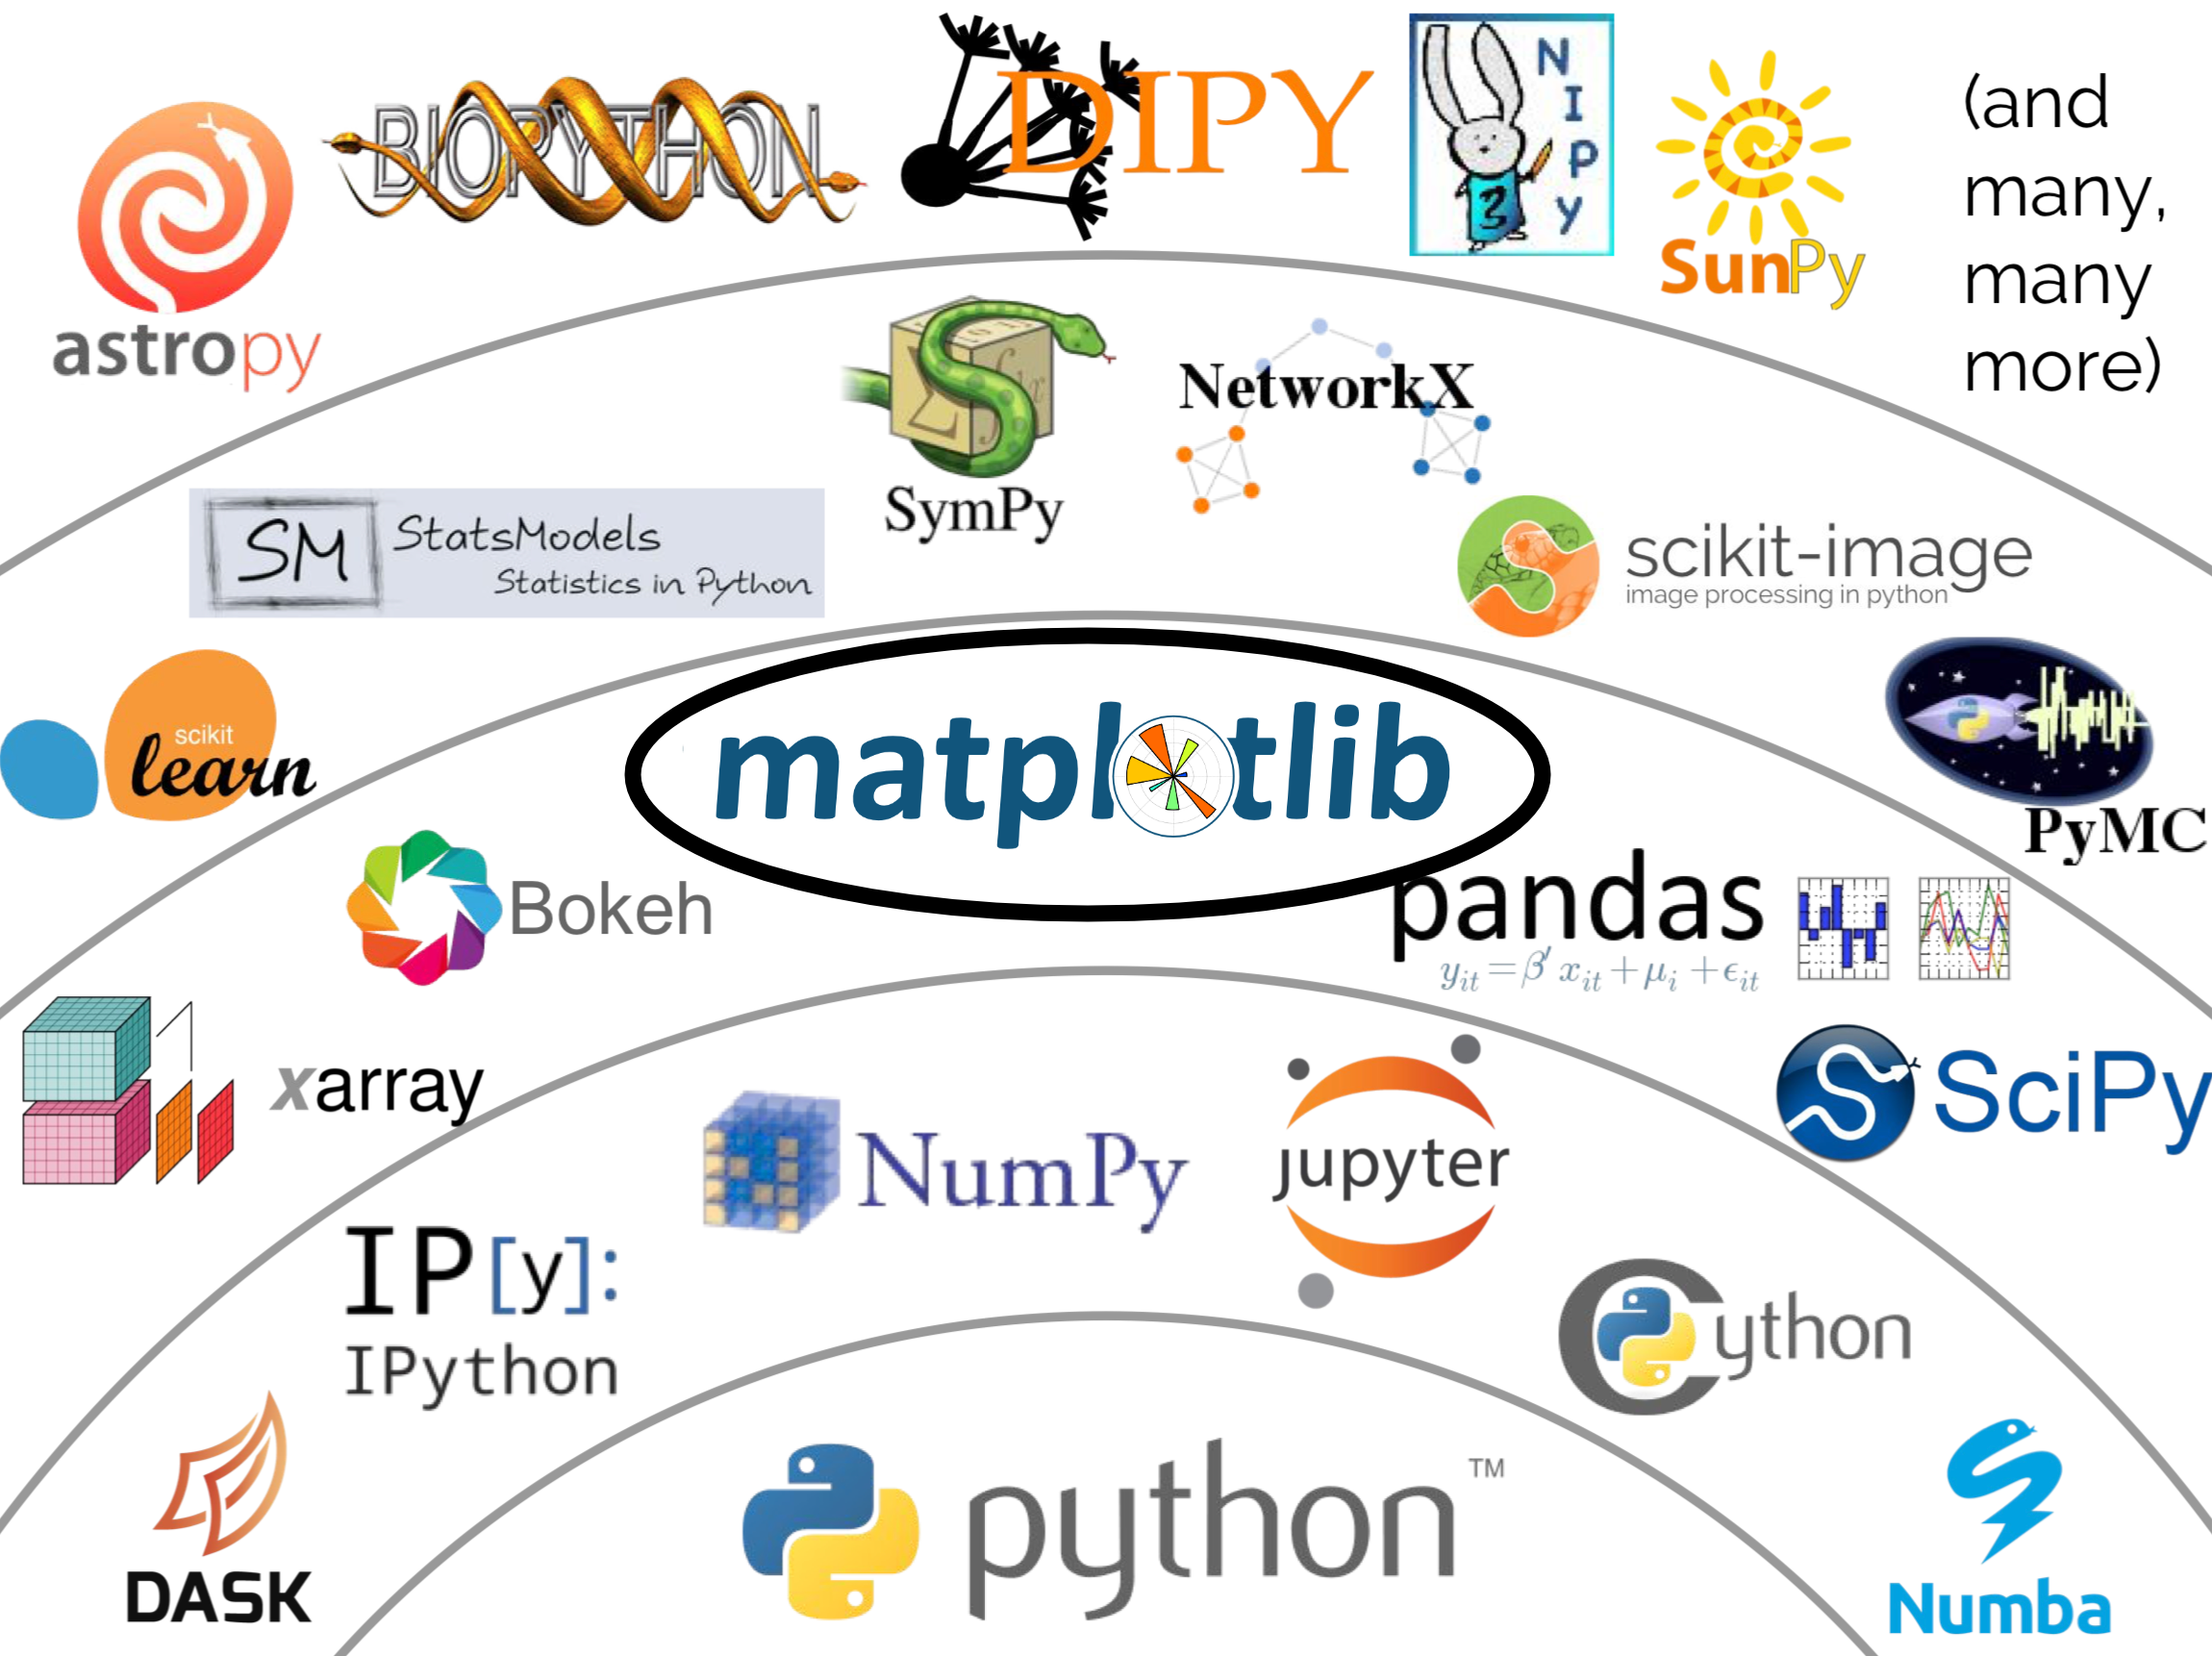
\includegraphics[width=0.45\textwidth]{scipy-ecosystem}
  \caption{A schematic of the Scientific Python ecossytem.  At the
    center we have the Python language itself with concentric rings of
    domain agnostic to domain specific libraries.  Both AstroPy (top
    left) and SunPy (top right), used in the astrophysics and
    heliophysics divisions respectively, rely on Matplotlib.
    Credit: Jake van der Plas, "The Unexpected Effectiveness of Python
    in Science", PyCon 2017}
  \label{fig:ecosystem}
\end{wrapfigure}



Matplotlib \cite{Hunter:2007} is an established open source plotting
library with a BSD-derived license that is currently used throughout
both the SMD science community and the wider scientific community.
The initial work on Matplotlib was done in 2001-2002 and the first
commits in the Matplotlib history date to early 2003.  Over the last
17 years Matplotlib has been actively developed and maintained by a
vibrant, primarily volunteer, community.  Matplotlib has over 1,250
individual contributors to the code base with countless more
individuals having contributed in ways not easily track, such as
answering user questions on the mailing list or reporting issues.

Matplotlib has a high-level API for quick plotting, such as in
exploratory data analysis, plus a low-level API that gives full control for
fine-tuned publication-quality plots, for animations, for writing both
GUI-independent and GUI-specific tools for interactive data plotting, and
for output to a variety of vector and raster
formats including \texttt{svg}, \texttt{eps},
\texttt{pdf}, and \texttt{png}

Matplotlib APIs as readily extendable.  The most common visualizations
in a domain need to be fluid for the end-practitioners, with the
``obvious'' customization options exposed. Much of the domain-specific
specialization is carried in the structure, semantics and assumptions
of the data, and in the standard visualizations of the domain. These
specializations can vary widely, in contradictory ways, between
domains. Because no high-level API can simultaneously satisfy all of
the visualization needs, there has developed a rich ecosystem of
domain specific plotting tools including yt, astropy, ArviZ,
seaborn, xarray, astropy, fast\_histogram extending the core
Matplotlib APIs.


While large parts of the scientific computing community rely on the
SPE, the open nature of these infrastructure tools makes measuring
their influence hard.  Conservative estimates, based on downloads and
web traffic on the documentation, are that Matplotlib has over a
million users.  Matplotlib is in top 100 most downloaded Python
packages from PyPI, and is packaged by every major Linux distribution.
We expect that a large fraction of NASA SMD-sponsored projects rely on
this shared infrastructure to some degree, but this is hard to prove
in practice.  In particular, scientific work does not usually cite the
software that was used for computation and plotting, and usage and
download statistics are hard to gather for widely used open source
packages.  Even though citation counts are likely to vastly
under-represent the scientific use of these packages, a canonical
reference for Matplotlib~\cite{Hunter:2007} has over 12,750 citations
while a common reference of NumPy\cite{walt2011numpy} has over 6,800
citations. These counts already illustrate a problem in measuring
usage via citations, as every user of Matplotlib also uses NumPy, but
Matplotlib has almost twice as many citations.  Domain specific tools,
like AstroPy~\cite{robitaille2013astropy} for astronomy (about 4,500
citations), often have high citation counts compared to the core
packages like NumPy, SciPy and Matplotlib that they are built upon.


\subsection{Objectives and Significance}


Matplotlib is a primarily community-driven project, but we have grown to the
point where we need supported developers with the time to organize, plan, and
make decisions.  To maintain Matplotlib's health we need to:
\begin{itemize}[noitemsep]
\item fix critical bugs and regressions;
\item triage the backlog of Issues and PRs in terms of topic,
  difficulty, and urgency and promptly triage newly opened Issues and
  PRs;
\item maintain backward compatibility and extensively document
  intentional changes;
\item on-board new contributors to sustain and diversify developer
  team;
\item maintain the CI infrastructure;
\item manage the release process;
\item and manage discussions about proposed enhancements, features,
  and API changes.
\end{itemize}
The requested support for developers is intended to complement and
facilitate, not replace, crucial volunteer work.  We aim to better
co-ordinate and nurture their efforts, with the goal of growing and
sustaining a diverse community of volunteer and paid expert
contributors.

[TODO remove or reword this?] Maintenance is inherently reactive, we
do not know about new bugs, user issues, or breaking changes in
upstream packages until they are reported gobto us.  While this critical
work can be done by volunteers, if we want to commit to a service
level we need paid developer time.

With supported developers we also be able to tackle larger scale
problems with the library that are too big to be done with volunteer
effort.  One such task is fully documenting, testing, and fixing (as
needed) the existing unit handling code in Matplotlib, which we
estimate to be 1.5FTE worth of effort by a single person and will
require long stretches of uninterpreted work time.


\subsubsection{Unit work}

Units are fundamental to science, however most numerical software is
unit-naive.  It the user's responsibility to keep track of and
correctly convert data to consistent units prior to any computation.
Failing to do so leads to the most insidious of bugs: everything
``works'' but silently gives incorrect results!  There are several
libraries which provide unit-aware data structures in Python and
Matplotlib, if passed these data structures, can use them for
unit-aware plotting.  This capability it is currently used to support
spaceflight operations by Monte, JPL's mission design and navigation
software system and the initial development was supported by NASA.

However, this support is under documented making it difficult for
users to understand and use the capability and for developers to
extend it.  Further, because we do not have 100\% test coverage to
verify that all the plotting methods correctly handle units we have
had a number of regressions, some still unresolved, in unit-aware
plotting.  We propose to write thorough user and developer guides to
working with unit-aware data in Matplotlib, add 100\% test coverage of
unit support in our plotting routines, and fix any issues and
inconsistencies discovered in this process.  Once we have documented
and fixed the existing functionality we will look into improving and
extending the user interface and API.

[TODO delete this paragraph?]  If Matplotlib detects units on user
input, we look up a conversion function to map from the unit-aware
data to unit-naive values we use internally.  Additionally we
configure the Axis to place ticks and format the tick labels.  By
default Matplotlib registers a converters for time and
string-categorical data and users and third-party libraries can
register their data structures and converters at run time to extend
this dispatch mechanism.

The first task is to document, both at the conceptual and API level,
how the unit dispatch system works in theory and how it works in
practice.  This documentation will be aimed at Matplotlib and
third-party library developers who want to use or extend the unit
system.  For unit-aware plotting to be effective, it must be available
on every plotting method so almost all Matplotlib maintainers will
need to be familiar with the mechanism.  Unfortunately, the original
authors of the unit-handling code are no longer active with the
project so we may have to reverse engineer some aspects of the code
and motivation.  Understanding and documenting how the unit-mechanism
was intended to work and the current state of the library and how it
will be the foundation of the rest of the work.

The second task is to write several user-facing tutorials making use
of the unit-full types we support by default and commonly used
down-stream unit libraries such as \texttt{unyt}
(\url{https://unyt.readthedocs.io/en/stable/}) and \texttt{pint}
(\url{https://pint.readthedocs.io/en/stable/}).  We will reach out to
current users, such as the Monte developers at JPL, and the AstroPy,
yt, and pandas developers, who depend on the unit machinery to ensure
that the examples are representative of how they use the functionality
in practice.  As with the developer documentation this will serve as
foundation for the rest of the work, however this documentation may be
prescriptive of the behavior we want to have rather than strictly
documenting the currently implemented behavior.

The third task is to ensure that all of the plotting methods support
unit-full data in a uniform way.  The documentation developed as part
of the first two tasks will guide how we resolve any inconsistencies.
We will address known bugs and inconsistencies and expect to find
additional bugs in the course of the work.  Fixing all of these issues
may require significant refactoring of the internal representation of
user data and will compliment the ongoing work to refactor the Artist
and data storage layers.

A final task is to extend the unit machinery to improve the user
experience.  Currently much of the mechanism of unit-handling is
implicit and automatic based on type inference.  We propose to extend
the interface to allow optional direct control of the unit machinery
by users and third-party library developers.  We will rely on the
documentation and testing from the previous work to ensure that we do
not introduce any new regressions or inconsistencies.



\subsubsection{General maintenance}


Historically, Pull Requests (PRs) and Issues are submitted faster than
they can be reviewed; Matplotlib has accumulated about 300 open PRs
1300 open Issues due to this imbalance, There may be critical bug
reports or insightful feature requests among the issue backlog, while
among the PR backlog are useful contributions or bug fixes that would
improve the libraries for direct users and downstream packages.  The
large backlog is discouraging for new and occasional contributors and
distracting for core developers.

There are a number of tasks that are required to ``keep the lights
on'' on a Python package include maintaining the continuous
integration systems, managing releases, tracking down
platform-specific bugs, and tracking upstream changes.  These are
tasks that are never ``done''; users find new ways to use the library
which require new features or expose previously un-detected bugs and
the world continues to changes around us.

For 10 months in 2020 we had a full time RSE working on Matplotlib who
had a measurable impact on both the rate of PR review, the rate of
issue resolution, and fixed a number of long standing bugs.  In 2020
Matplotlib resolved 125-200 PRs and 75-125 Issues a month, however
even with this dedicated effort we only reduced the PR backlog by 70
open PRs and made no progress on reducing the Issue backlog.  The
additional resources requested will help to significantly reduce, but
not eliminate, this backlog.

\subsection{Perceived impact of work}
\begin{enumerate}
\item increased reliability of unit-aware plotting
\item improvement in general reliability of software
\item improved responsively to issues
\end{enumerate}
\subsection{Relevance to program element}

As mentioned above, it is hard to estimate the prevalence of open
source software due to it being freely distribute and not
systematically cited.  Matplotlib is in the top 100 most-downloaded
packages from PyPI\cite{pypi_stats} and is packaged by every major
Linux and scientific Python distribution.  One path is static analysis
of publicly available code.  According to github over 299K
repositories and over 12k packages hosted on Github depend on
Matplotlib\cite{gh_deps:2021} and a recent study of the almost 10M
Jupyternotebooks on github found that over 3M of them have a
Matplotlib import\cite{datalore:2020}.

All of these measures show broad impact but cover many uses outside of
the SMD community.  Restricting static analysis to
\url{https://github.com/nasa} shows usage of Matplotlib, however this
does not capture the wider user base.  Soliciting for examples of
Matplotlib in SMD research on social media yielded a (non-exhaustive)
list of examples of using Matplotlib
\begin{itemize}
\item
  to study
  thunderstorms\cite{https://doi.org/10.1002/2016JD025299,https://doi.org/10.1029/2019JD030874},
  seasonal ocean winds \cite{https://doi.org/10.1002/2017JD027516} and
  tropical storms \cite{Lang_2020};
\item in the first science paper from the Parker Solar
  probe\cite{Bale2019};
\item in the Martian science program in both orbiter
  \cite{https://doi.org/10.1029/2019JE006188} and
  rover\cite{https://doi.org/10.1002/2016EA000219} contexts;
\item as part of ground operations from the Phoenix Lander;
\item with data from Kepler and K2 missions to study Trojan
  asteroids\cite{Nixon_2019} and Titan
  \cite{Ryan_2017,2019PASP..131h4505P};
\item on the New Horizons Kuiper belt extended mission
  \cite{Porter_2018};
\item for visualization of scheduling, safety and constraint checks,
  and telemetry by the Swift science operations team
  \cite{swift_ops,2020ApJ...900...35T};
\item as port of the Hubble Space Telescope and James Web Space
  Telescope data processing pipelines;
\item in Monte, JPL's mission design
  and navigation software system to support spaceflight operations;
\item in fundamental research on graphene \cite{PhysRevLett.120.236802};
\item and for work on nuclear rockets \cite{leu_cerment}.
\end{itemize}
This list shows the breadth of the use of Matplotlib across the
four SMD divisions.  Small investments in Matplotlib will have returns
across the entire SMD portfolio.

\subsection{Technical approach and methodology}

our standard practice!

\subsection{sources of uncertainty/mitigation to risk}


The biggest risk with the proposed work is that we are underestimating
the amount of work that will be required for the unit work.  There is
always a risk while refactoring that the scope of work rapidly snow
ball due to unexpected internal dependencies or edge cases must be
accounted for.  In a worst case where we have to abandon the work we
will maintain the status quo, but with significantly better
documentation.

We anticipate that all of the work can be done incrementally and will
be merged to the default branch of Matplotlib throughout the
performance period.  This is inline with our standard development
process, work done under this proposal will not be exempt from review,
and many small PRs are easier to review and merge than a single large
PR.  This process inherently reduces the risk as we will be frequently
merging improvements to the default branch.  These These improvements,
both to the code and documentation, will in turn be released to users
as part of our standard bi-yearly release cadence.

There is very little risk in the maintenance work.  There is large
volume of individually small tasks that need to be addressed: the
issue and PR backlogs.  Any dedicated effort devoted to clearing the
backlog is positive and we have demonstrated that supported developers
can reduce, or at least hold even, the backlogs.


\subsection{roles of team members}
\begin{enumerate}
\item Caswell: PI + maintenance + supervise RSE (0.25FTE)
\item RSE: maintenance + lead unit unit testing (1FTE)
\end{enumerate}

\subsection{workplan with milestones}

Starting from July 2021 onward Dr. Caswell will devote 25\% FTE to
this work.  This time will be split between supervision of the RSE and
maintenance work, both of these are on-going tasks.  The first task
will be the recruitment and hiring of the RSE.

The Research Software Engineer (RSE), whom needs to be identified,
will devote 100\% FTE to this project.  This will be split evenly with
50\% FTE being spent on the unit work and 50\% being spent on general
maintenance until the unit work is complete.  If the unit work is
completed faster than expected, the RSE will devote 100\% of their
effort to maintenance.  Because Matplotlib is a community project, the
work of the RSE will still go through the normal review process.  The
interaction with community makes it advantageous to spread out the
unit work.  The first task, producing developer-facing documentation
about how the unit system works we expect to take 25\% FTE with will
be spread across the first two quarters of the grant.  Similarly,
writing the user-facing documentation should take about 25\% FTE which
will be done is the third and forth quarters of the performance
period.  The remaining work on units, adding the tests, fixing any
bugs and inconsistencies, and any required internal refactoring, will
take 1 FTE spread across final 2 years of the performance period.
Incremental progress will be merged and released as part of the normal
release cycle throughout the performance period.  The RSE will present
the status of the work at two conferences, expected to be SciPy in
July and one of PyData conferences in the winter, yearly.


\begin{description}

\item[Y1Q1] Begin first units task (documenting current behavior)
\item[Y1Q2] Finish first task. Have developer documentation merged to
  Matplotlib docs.
\item[Y1Q3] Begin second task.
\item[Y1Q4] Finish second task. Have user-facing documentation merged
  to Matplotlib docs. Present at SciPy and/or pydata.

\item[Y2Q1] Begin third task.  Develop detailed development plan.
\item[Y2Q2] Continue third task.
\item[Y2Q3] Continue third task.
\item[Y2Q4] Present at SciPy and/or pydata.


\item[Y3Q1] Continue third task. Evaluate progress on development
  plan, adjust if needed.
\item[Y3Q2] Continue third task.
\item[Y3Q3] Continue third task.
\item[Y3Q4] Completed third task. Present at SciPy and/or pydata.

\end{description}



\subsubsection{Grant Management Plan}

Dr. Caswell of BNL is the PI of the proposed development and is the
Matplotlib Lead Developer.  He is solely responsible for the quality
and direction of the proposed work and the proper use of all awarded
funds.  He is also responsible for all management, and budget issues
and is the final authority for this task.


\subsection{Project Management}
\subsubsection{Governance}
Matplotlib is a NumFOCUS Fiscally Sponsored Project.  The governance
is specified at
\url{https://github.com/matplotlib/governance/blob/master/governance.md}.
The project has a Project Lead (Caswell) who is the final authority in
all decisions, however when possible all decisions are made by
community consensus.  In addition to the Project Lead, there is a
formalized Steering Council which is responsible for the overall
direction of the project, and several Deputy Project Leads who have
day-to-day technical responsibilities.

TODO need to cover history of project lead changing

\subsubsection{License}

BSD-derived

\subsubsection{sustainability metrics}
\begin{enumerate}
\item Continue Regular releases (mpl minor every 6mo, patch every 2mo
  or as needed).
\item Increase number of new regular contributors
\item Rate of PR / Issue throughput
  \begin{enumerate}
  \item caveats on how issues/PRs are very varied in time to resolve
  \end{enumerate}
\end{enumerate}

\subsubsection{collaboration with related projects}

None of the projects in the Scientific Python ecosystem existing in a
vacuum; a vast majority of our users use more than one of the
projects.  In a mirror of that, while developer communities exist
around each of the code bases, there is also a broader developer
community across the projects.  Matplotlib developers are part of this
community and have well established relationships with the other
projects in the ecosystem, including our key up and down stream
dependencies.

Much of the communication is through the standard communication
channels, such as project issue trackers, mailing lists or discussions
forums, and submitting PRs.  The strongest relationships, both
historical and current, are with projects where we have shared
developers.  For example Ryan May and Elliot sales de Andre are both
core contributors to Matplotlib and Cartopy.  Micheal Droettboom, the
previous Matplotlib Project lead, was a core developer on Astropy.
Additionally, through NumFOCUS and domain-specific conferences there
are regular in-person meetings.

[TODO not sure where this fits?] Almost all of the Matplotlib
contributors, are domain experts in their primary domain and use
Matplotlib for their research.


% wording all NF projects are putting in
As a NumFOCUS project, we recognize the importance of every project
that is part of our open source scientific computing community. Though
we would like for our work to be funded we are committed to supporting
and collaborating with other NumFOCUS projects that receive funding
regardless of our own outcome. We believe that this attitude is
crucial for the success of our community and the sustainability of
open source projects. It is our hope that this sentiment will be taken
into consideration when evaluating our proposal.


\subsubsection{inclusive practices}

Matplotlib strives to be an inclusive and open project and have
adopted a Code of Conduct
\url{https://github.com/matplotlib/matplotlib/blob/master/CODE_OF_CONDUCT.md}. Anyone
who is willing and able to contribute to the project should feel
welcome to do so.  It is important for everyone working on the project
to feel safe to make mistakes.

We have recently started two efforts to improve the development and
retention of new contributors: an ``incubator'' channel on gitter and
a Triage Team.

The hardest part of getting started to contributing to open source
projects is can be simply getting started.  The incubator is a
semi-closed chat room where new contributors can get support on any
aspect of contributing to Matplotlib.  This include the technical
aspects of the code they are working on, help with git/github, our
review process, or the social expectations and norms of the community.  The
goal is that by providing this support to first time contributors we will
retain more of them as regular contributors and then maintainers.

The issue tracker is important to communication in the project because
it serves as the centralized location for making feature requests,
reporting bugs, identifying major projects to work on, and discussing
priorities.  For this reason, it is important to curate the issue
list, adding labels to issues and closing issues that are resolved or
unresolvable. Triaging issues does not require any particular
expertise in the internals of Matplotlib but is extremely valuable to
the project.  To this end we have created a ``Triage Team'' in the
organization who have power to tag, milestone, and close issues.  In
addition to the direct benefit of improving the issue triage and
freeing the core-developers to spend more time reviewing PRs, this
role will bring more people into the developer community and may
provide a path way to becoming regular contributors and maintainers.

One challenge of being an open community developed project is that we
do not have reliable demographics on a vast majority of our
contributors.  Ongoing work at NumFOCUS to develop metrics will help
us evaluate the efficacy of these efforts at diversifying our
contributor base.

\subsubsection{information dissemination}

As a project Matplotlib maintains a range of communication channels
aimed at several, overlapping, audiences.  This includes a
the source, issue tracker and PRs on GitHub,
the published documentation (inculding historical and ``future'' versions),
weekly developer call,
mailing lists,
a discourse forum,
an active chat room on gitter,

in-person presentations at conferences and pydata events,
a blog, and several social media accounts.


The center of gravity of Matplotlib development takes place on GitHub
(\url{https://github.com/matplotlib/matplotlib}) where the canonical
repository for the source and documentation are hosted.  Around this
repository we use Issues and PRs to track bug reports, feature
requests, and to discuss proposed changes.  We also host our
governance documents on GitHub
(\url{https://github.com/matplotlib/governance}) and revise them via
Pull Request.

We publish extensive prose, example, and API documentation
(\url{https://matplotilb.org}) that is refreshed with each release.
In addition to the top-level docs, which always refer to the most
recent release, we also host historical
(\url{https://matplotilb.org/3.1.3} for the v3.1.3 documentation) and
development versions of the documentation
(\url{https://dev.matplotilb.org}).  In 2020 we had between 700k-1M
unique visitors a month to the documentation.


The weekly developer calls are typically attended by six to eight
people and are used for high-bandwidth discussions about both the
overall direction of the project and technical issues depending on the
day.  The agenda and minutes are publicly available
(\url{https://hackmd.io/team/matplotlib}) and the calls are open to
all.

Matplotlib has an active gitter
(\url{https://gitter.im/matplotlib/matplotlib}) chat room.  Gitter is
a real-time chat platform that we use for general coordination and
resolving minor technical discussions.  While the chat room's history
is technically persistent, we treat it as transient.  For more in
depth discussions or anything we want a record of, we move the
conversation to github, the mailing list, or discourse.

For user support and general discussion we maintain two mailing lists
(\url{https://mail.python.org/mailman/listinfo/matplotlib-users},
\url{https://mail.python.org/mailman/listinfo/matplotlib-devel}) and a
discourse (\url{https://discourse.matplotlib.org}) instance.  While
users have to subscribe and register respectively to post, these
forums are open to all.  We also maintain a read-only mailing list for
announcements
(\url{https://mail.python.org/mailman/listinfo/matplotlib-announce}).

When we could travel Matplotlib developers would frequently attend
in-person meetings including SciPy and PyData events.

We have a blog (\url{https://matplotlib.org/matplotblog/}) which hosts
user-submitted content highlighting work they have done using
Matplotlib.  We have project accounts on several social media platform
including twitter and Instagram.


\subsection{current workflow}

Matplotlib is an established community driven project in the
``federation'' model as defined by Nadia Eghbal\cite{eghbal_2020}.  We
have a core group regular maintainers who take responsibility for
reviewing and merging proposed changes to the library.  We strive for
consensus and rely on the collective judgment of our maintainers to maintain
the quality and functionality of the library.

Matplotlib uses a variation on the ``git flow'' process
(\url{https://guides.github.com/introduction/flow/}) to manage
proposing and reviewing contributions to the library and documentation
though on GitHub
(\url{https://matplotlib.org/devel/coding_guide.html}).  A
contributor, a core maintainer, a regular contributor, or a first time
contributor, proposes a change by opening a ``Pull Request'' from
their fork of Matplotlib.  The proposed changes are reviewed by
maintainers who either request changes, which starts a cycle of
iteration with the contributor, or approve.  In addition to human
review we have an extensive test suite that is automatically run via
cloud services and the results are reported to the PR.  Once consensus
is reached and the test pass the PR is merged and the changes will be
released as part of the next release.

The threshold for merging a PR depends on the reviewer judgment of the
risk of the changes.  PRs that only change documentation, which cannot
introduce regressions or introduce new features, may be merged by the
first reviewer where as code changes need to be reviewed and approved
by at least two maintainers.  However in either case a maintainer may
wish to leave a positive review but not merge the PR to request
additional feed back from other maintainers.  If a maintainer objects
to a PR, the PR will not be merged until their concerns have been
addressed.  If consensus cannot, the final decision falls back to a
Deputy Project Lead or the Project Lead.

Matplotlib is cautious about making backwards-incompatible change that
intentionally break users existing code.  While in an ideal world,
future versions of the library would be 100\% backwards compatible
with previous versions, sometimes we do need to make incompatible
changes.  As part of the review process we check that any API changes
are well documented and justified.  When technically possible we
provide user-visible warnings the version before we actually implement
a breaking change.  This provides a window for users to either adapt
to the change or to communicate to us that they cannot adapt so we
can reconsider the change.  Given this high barrier to changing or
removing behavior we are careful to make sure that any new API we add
to the library is well thought out and complete because once we have
released a version of the library with that code it is hard to take it
back.  These considerations together are important enough that we have
a Deputy Project Lead responsible for API consistency.

This process works well for incremental contributions and bug fixes,
new features or bigger changes are typically discussed before
significant work is done.  In many cases if the feature does not need
to be in the core library we encourage contributors to create a new
stand-alone project.  This has several advantages including the giving
the author more control, allows them to iterate faster than our
relatively slow 6 month release schedule, and gives them greater
flexibility to change their APIs.


\newpage
% Here's how I get references.
% needed for AAS citation

\def\ref@jnl#1{{\rm#1}}

\def\aj{\ref@jnl{AJ}}                   % Astronomical Journal
\def\actaa{\ref@jnl{Acta Astron.}}      % Acta Astronomica
\def\araa{\ref@jnl{ARA\&A}}             % Annual Review of Astron and Astrophys
\def\apj{\ref@jnl{ApJ}}                 % Astrophysical Journal
\def\apjl{\ref@jnl{ApJ}}                % Astrophysical Journal, Letters
\def\apjs{\ref@jnl{ApJS}}               % Astrophysical Journal, Supplement
\def\ao{\ref@jnl{Appl.~Opt.}}           % Applied Optics
\def\apss{\ref@jnl{Ap\&SS}}             % Astrophysics and Space Science
\def\aap{\ref@jnl{A\&A}}                % Astronomy and Astrophysics
\def\aapr{\ref@jnl{A\&A~Rev.}}          % Astronomy and Astrophysics Reviews
\def\aaps{\ref@jnl{A\&AS}}              % Astronomy and Astrophysics, Supplement
\def\azh{\ref@jnl{AZh}}                 % Astronomicheskii Zhurnal
\def\baas{\ref@jnl{BAAS}}               % Bulletin of the AAS
\def\bac{\ref@jnl{Bull. astr. Inst. Czechosl.}}
                % Bulletin of the Astronomical Institutes of Czechoslovakia
\def\caa{\ref@jnl{Chinese Astron. Astrophys.}}
                % Chinese Astronomy and Astrophysics
\def\cjaa{\ref@jnl{Chinese J. Astron. Astrophys.}}
                % Chinese Journal of Astronomy and Astrophysics
\def\icarus{\ref@jnl{Icarus}}           % Icarus
\def\jcap{\ref@jnl{J. Cosmology Astropart. Phys.}}
                % Journal of Cosmology and Astroparticle Physics
\def\jrasc{\ref@jnl{JRASC}}             % Journal of the RAS of Canada
\def\memras{\ref@jnl{MmRAS}}            % Memoirs of the RAS
\def\mnras{\ref@jnl{MNRAS}}             % Monthly Notices of the RAS
\def\na{\ref@jnl{New A}}                % New Astronomy
\def\nar{\ref@jnl{New A Rev.}}          % New Astronomy Review
\def\pra{\ref@jnl{Phys.~Rev.~A}}        % Physical Review A: General Physics
\def\prb{\ref@jnl{Phys.~Rev.~B}}        % Physical Review B: Solid State
\def\prc{\ref@jnl{Phys.~Rev.~C}}        % Physical Review C
\def\prd{\ref@jnl{Phys.~Rev.~D}}        % Physical Review D
\def\pre{\ref@jnl{Phys.~Rev.~E}}        % Physical Review E
\def\prl{\ref@jnl{Phys.~Rev.~Lett.}}    % Physical Review Letters
\def\pasa{\ref@jnl{PASA}}               % Publications of the Astron. Soc. of Australia
\def\pasp{\ref@jnl{PASP}}               % Publications of the ASP
\def\pasj{\ref@jnl{PASJ}}               % Publications of the ASJ
\def\rmxaa{\ref@jnl{Rev. Mexicana Astron. Astrofis.}}%
                % Revista Mexicana de Astronomia y Astrofisica
\def\qjras{\ref@jnl{QJRAS}}             % Quarterly Journal of the RAS
\def\skytel{\ref@jnl{S\&T}}             % Sky and Telescope
\def\solphys{\ref@jnl{Sol.~Phys.}}      % Solar Physics
\def\sovast{\ref@jnl{Soviet~Ast.}}      % Soviet Astronomy
\def\ssr{\ref@jnl{Space~Sci.~Rev.}}     % Space Science Reviews
\def\zap{\ref@jnl{ZAp}}                 % Zeitschrift fuer Astrophysik
\def\nat{\ref@jnl{Nature}}              % Nature
\def\iaucirc{\ref@jnl{IAU~Circ.}}       % IAU Cirulars
\def\aplett{\ref@jnl{Astrophys.~Lett.}} % Astrophysics Letters
\def\apspr{\ref@jnl{Astrophys.~Space~Phys.~Res.}}
                % Astrophysics Space Physics Research
\def\bain{\ref@jnl{Bull.~Astron.~Inst.~Netherlands}}
                % Bulletin Astronomical Institute of the Netherlands
\def\fcp{\ref@jnl{Fund.~Cosmic~Phys.}}  % Fundamental Cosmic Physics
\def\gca{\ref@jnl{Geochim.~Cosmochim.~Acta}}   % Geochimica Cosmochimica Acta
\def\grl{\ref@jnl{Geophys.~Res.~Lett.}} % Geophysics Research Letters
\def\jcp{\ref@jnl{J.~Chem.~Phys.}}      % Journal of Chemical Physics
\def\jgr{\ref@jnl{J.~Geophys.~Res.}}    % Journal of Geophysics Research
\def\jqsrt{\ref@jnl{J.~Quant.~Spec.~Radiat.~Transf.}}
                % Journal of Quantitiative Spectroscopy and Radiative Transfer
\def\memsai{\ref@jnl{Mem.~Soc.~Astron.~Italiana}}
                % Mem. Societa Astronomica Italiana
\def\nphysa{\ref@jnl{Nucl.~Phys.~A}}   % Nuclear Physics A
\def\physrep{\ref@jnl{Phys.~Rep.}}   % Physics Reports
\def\physscr{\ref@jnl{Phys.~Scr}}   % Physica Scripta
\def\planss{\ref@jnl{Planet.~Space~Sci.}}   % Planetary Space Science
\def\procspie{\ref@jnl{Proc.~SPIE}}   % Proceedings of the SPIE

\let\astap=\aap
\let\apjlett=\apjl
\let\apjsupp=\apjs
\let\applopt=\ao
\setcounter{page}{1}
\bibliography{mpl_cartopy.bib}

\newpage
\section{Data Management Plan}
\setcounter{page}{1}

Matplotlib is a software library and does not produce any scientific
data as defined in E.1.2 that needs to be preserved.

Matplotlib is currently developed in the open on GitHub and is
released under a permissive license (the Matplotlib license which is a
derivative of the PSF license and compatible with BSD-3).  All work
done on Matplotlib as part of this grant will be done through the
current workflow, will be publicly available, and released under the
same license.  Matplotlib uses git for version control, thus every
developer has the full history on their computer which provides
significant redundancy.  Tagged releases of the software are published
to PyPI (in both source and binary forms).  In addition, Anaconada,
macports, homebrew, and all major Linux distributions independently
build, package, and host Matplotlib.  User facing documentation is built
and hosted at \url{https://matplotlib.org}.

%do we need something about shape files / map tiles?

Any new libraries created as part of the ROSES award will be developed
in the open on GitHub and will released under a BSD-3 license.

% do we need this?
Any incidental work on other software packages, either upstream or
downstream of Matplotlib, will have to follow the license and
development of process of those projects.


\newpage
\section{Biographical Sketches}
\setcounter{page}{1}
\subsection{Principal Investigator}
\newpage
\subsection{Co-Investigator}

% This line gets the space in TOC right.
\addtocontents{toc}{\protect\vspace{12pt}}
\newpage
\section{Table of Personnel and Work Effort}
\setcounter{page}{1}

\newpage
\section{Current and Pending Support}
\setcounter{page}{1}

\newpage
\section{Budget Justification}
\setcounter{page}{1}

Due to being an established community driven project most regular
contributors have established and distinct primary institutions.  For
this reason significant portions of the budget will need to be
subcontracted to the primary institutions of key individuals who are
uniquely qualified for this work.

Salary support is requested for PI Thomas Caswell (0.25 FTE in years
1-3).  He will oversee the Matplotlib aspects of the proposed work and
co-supervise the RSE.

Salary support is requested for a Research Software Engineer (1 FTE in
years 1-3).  The RSE will be responsible for carrying out the unit
work on Matplotlib and general maintenance tasks on both Matplotlib
and Carotpy.

Support is requested for the RSE to attend the SciPy conference in
Austin, TX each year.  Cost estimates are based on the following: Meal
per diem from the GSA website, airfare from NYC to ATX from
\url{https://travel.google.com}, 2019 registration and conference hotel.

\begin{description}
\item[airfare] \$500
\item [lodging] \$770 (5 nights at \$154/night)
\item [Registration] \$700
\item [per diem] \$396 (\$61/day)
\item [misk ground transport] \$100
\item [total for one person] \$2,466
\end{description}

Support is requested for the RSE to attend a PyData conference
someplace in the USA each year.  Cost estimates are based on the
following: Meal and hotel per diem from the GSA website for NYC in
November (as a worst-case scenario), airfare from NYC to LAX from
\url{https://travel.google.com}, and guidance from NumFOCUS as to the
registration fee.


\begin{description}
\item [airfare] \$500
\item [lodging] \$858 (3 nights at \$286/night)
\item [Regisration] \$200
\item [per diem] \$342 (\$76/day)
\item [misk ground transport] \$100
\item [total for one person] \$1,800
\end{description}


Total requested for travel: \$12,798


\newpage
\section{Facilities and Equipment}
\setcounter{page}{1}

Standard desktop workstations that Caswell has access to, either
through BNL or personal hardware, is sufficient for this work.

We request \$4,000 to purchase a computer, monitor, and accessories
for the RSE.


[TODO do we want to ask for any CI / hosting budget here?]



\newpage
\section{Detailed Budget}
\setcounter{page}{1}




\end{document}
